\chapter{Einleitung}
\label{chap:Einleitung}
In allen sich mit Phänomenen und Gegenständen der erfahrbaren Außenwelt beschäftigenden Bereichen von Wissenschaft und Industrie ist das Vermessen eben jener Gegenstände von höchstem Interesse. Die Messtechnik als Schnittstelle zwischen der empirischen und der mathematisch-quantifizierten Welt ermöglicht erst als solche das Aufstellen und Validieren von Modellen, welche erfahrene Realitäten abbilden sollen. Es überrascht also nicht, dass gerade im Zuge von technologischem Fortschritt auch immer neue Methoden und Möglichkeiten gesucht werden, Objekte von Interesse zu vermessen. \newline
Eine dieser (realtiv) neuen Methoden besteht in dem Abtasten von Objekten mittels eines Lasers. Dieses Verfahren wurde zuerst in den 60er Jahren erfolgreich eingesetzt, auch wenn die ersten industriellen Anwendungen noch ca. 20 Jahre auf sich warten ließen (vgl. \cite{Ebrahim:11}). Dabei wird ein Laser auf ein zu vermessendes Objekt projiziert und mittels der räumlichen Informationen, die über den Laseremitter an sich, die Laserprojektion oder den Blickwinkel des Betrachters der Projektion bekannt sind, wird eine Distanzvermessung vorgenommen. Welche dieser Informationen wie verarbeitet wird, hängt von dem eingesetzten Verfahren ab. Bei den meisten Verfahren werden aus genügend gesammelten Distanzen dann 3D-Modelle des zu vermessenden Objektes angefertigt. Man spricht dann von einem 3D-Laserscanning. \newline
Industrielle Laserscanner werden heutzutage in vielen Bereichen der Vermessungstechnik benutzt und sind von der Minenvermessung (vgl. \cite{riegl:17}) bis zur Forensik (vgl. \cite{Zoller:16}) in allen möglichen Anwendungsbereichen vertreten. Diese Scanner weisen eine hohe Genauigkeit auf, sind für Privatpersonen meistens jedoch zu teuer. Da jedoch auch die Funktionsweisen von professionellen Laserscannern fundamentalen Prinzipien folgen, sind die an sich eingesetzten Verfahren vergleichsweise leicht nachzuvollziehen. Daher wurde für die vorliegende Ausarbeitung der Versuch unternommen, einen "`Do It Yourself''-Laserscanner zu bauen. Dieser soll das Lichtschnittverfahren als eine konkrete Art des Laserscannings erfolgreich mit Hilfe von Matlab als Entwicklungsumgebung umsetzen. In der Implementierung ist die Konstruktion einer Scan-Vorrichtung, die zugehörige Software und das Durchführen des Vermessungsverfahrens an sich enthalten. Es wurde vor allem auf die Einhaltung folgender Design-Prinzipien geachtet:
\begin{description}
\item[Simplizität] \hfill \\
Der Scanner sollte einfach zu konstruieren und zu bedienen sein. Außerdem sollten sich sowohl die Berechnungen als auch die Software, in der besagte Berechnungen stattfinden, leicht nachvollziehen lassen. Dies macht den Umgang mit dem Scanner komfortabler und begünstigt Nachbauten.
\item[Bezahlbarkeit] \hfill \\		
Der Scanner sollte preisgünstig konstruierbar sein und auch ohne High-End-Komponenten akzeptable Ergebnisse liefern.  
\item[Genauigkeit] \hfill \\  		
Ohne genaue Ergebnisse ist das Unterfangen einer Vermessung unnütz. Daher muss der Laserscanner unter der Annahme einiger Randbedingung möglichst genaue und reproduzierbare Messergebnisse liefern, welche das gemessene Objekt gebührend präzise als 3D-Modell abbilden.
\end{description}
In den folgenden Kapiteln wird zuerst auf die mathematische Theorie des Lichtschnittverfahrens eingegangen. Es folgt die konkrete Implementierung und die Beschreibung, wie der Scanner konstruiert wurde und wie bei einem einzelnen Scanvorgang die Vermessung und Datenverarbeitung durchgeführt wird. Anschließend werden die Ergebnisse begutachtet und es wird erläutert, wie erfolgreich die Hauptbearbeitungsschritte der Laserlinienerkennung und Koordinatenberechnung sind und warum. Geschlossen wird mit einem Fazit, welches alternative Techniken sowie mögliche weiterführende Schritte und Verbesserungen anführt.  

\begin{figure}
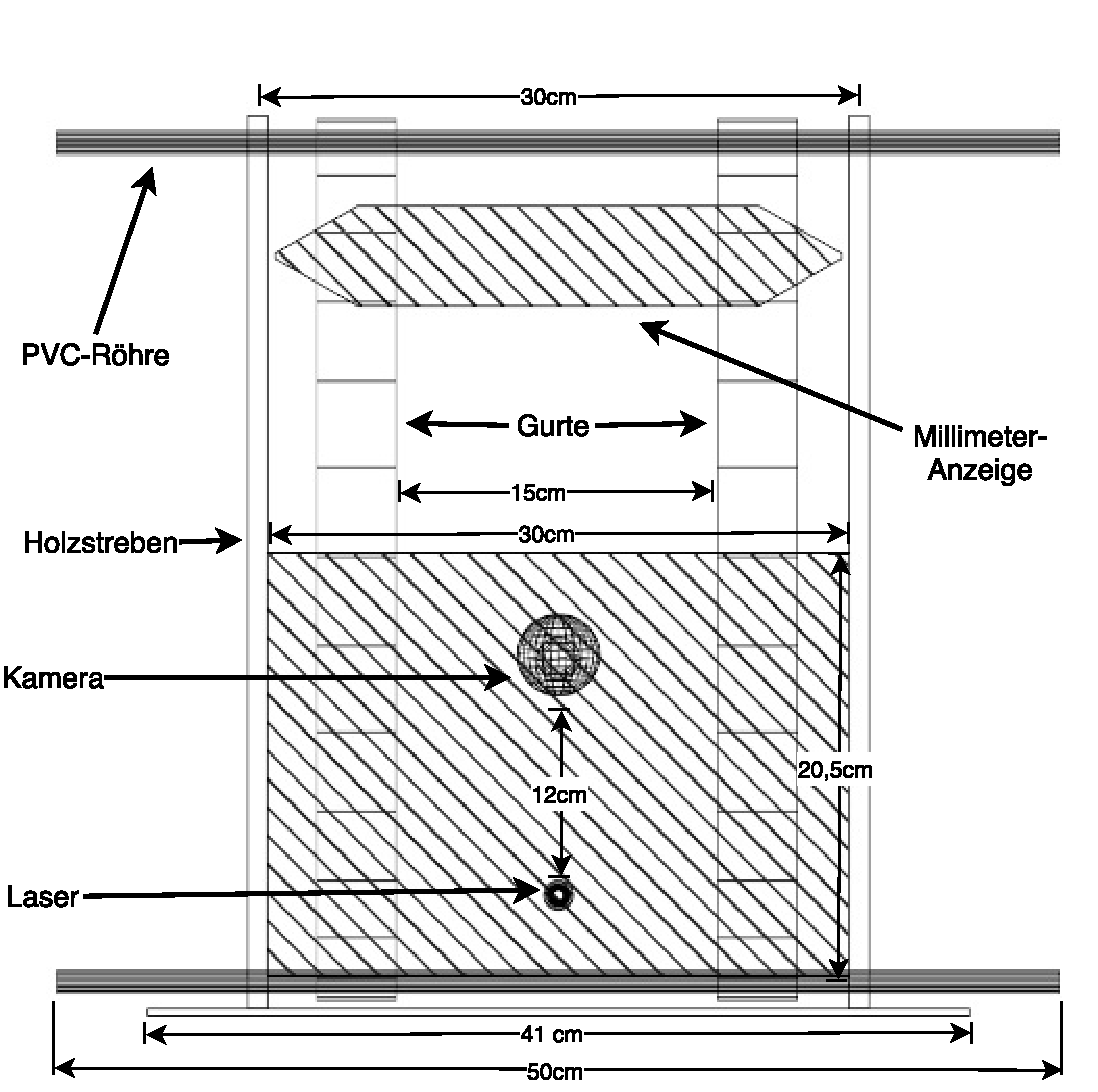
\includegraphics[width=\textwidth]{images/test.pdf}
\caption{Die Stufen des Scanvorgangs schematisch dargestellt}
\end{figure}

